\documentclass[11pt,a4paper,twoside,italian]{book}
\usepackage[italian]{babel}
\usepackage[T1]{fontenc}
\usepackage[utf8]{inputenc}
%\usepackage[italian]{babel}
\usepackage{DTGtesi}
%\usepackage{latexsym}
\usepackage{booktabs}
% Pacchetto per l'inserimento del codice Matlab
\usepackage{mcode}
\lstloadlanguages{MATLAB}
\usepackage{xcolor}
%\usepackage{listings}
%\lstset{language=Matlab}
% Pacchetto per l'inserimento delle formule matematiche
%\usepackage{amsmath}
\usepackage{amsmath,amssymb}
%\usepackage{amsthm}
\newcommand{\numberset}{\mathbb}
%\newcommand{\C}{\numberset{C}}
\newcommand{\R}{\numberset{R}}
\usepackage{subfigure}
\usepackage{caption}

%%%aggiunti io
\usepackage{hyperref}
\newcommand{\mail}[1]{\href{mailto:#1}{\texttt{#1}}}
\newtheorem{definizione}{Definizione}
\newtheorem{teorema}{Teorema}
\usepackage{amsmath}
\usepackage{algorithm}
\usepackage[noend]{algpseudocode}
\usepackage{lipsum}
\usepackage{pdfpages}
\usepackage{cite}
\newcommand*{\rom}[1]{\expandafter\@slowromancap\romannumeral #1@}
\newcommand{\RNum}[1]{\uppercase\expandafter{\romannumeral #1\relax}}
\usepackage[normalem]{ulem}
\useunder{\uline}{\ul}{}
\usepackage{float}

\bibliographystyle{unsrt}


\hypersetup{
  % pdfpagelayout=SinglePage, % default
  % pdfpagemode=UseOutlines,  % default
  % bookmarksopen,            % default
  % bookmarksopenlevel=2,     % default
  linkcolor=black,
  pdftitle=Proprietà di scala della biodiversità in comunità microbiche,
  pdfauthor=Eleonora Manoli,
  pdfsubject=Tesi di Laurea in Fisica,
  pdfkeywords=tesi laurea triennale}
  
%%%%%%%
  % Queste informazioni non vengono stampate, ma sono conservate nel documento pdf. Sono consultabili col menu "File>Document Properites>Description". Vengono buone a scopi archivistici.

%%%%%%%%%%%%%%%%%%%%%%%%%%%%%%%%%%%%%%%%%%%%%%%%%%%%%%%
%          Numerazione delle formule                  %
% Se non specificato altrimenti, il LaTeX numera le   %
% formule come (capitolo.formula) (per esempio (2.5)  %
% e` la quinta formula del secondo capitolo).         %
% Con le istruzioni seguenti invece la numerazione    %
% diventa (capitolo.sezione.formula) (per esempio     %
% (3.2.6) e` la sesta formula della seconda sezione   %
% del terzo capitolo):                                %
%%%%%%%%%%%%%%%%%%%%%%%%%%%%%%%%%%%%%%%%%%%%%%%%%%%%%%%

%\makeatletter
%\@addtoreset{equation}{section}
%\makeatother
%\renewcommand{\theequation}%
% {\thesection.\arabic{equation}}

%%%%%%%%%%%%%%%%%%%%%%%%%%%%%%%%%%%%%%%
% Dati per la prima pagina della tesi %
%%%%%%%%%%%%%%%%%%%%%%%%%%%%%%%%%%%%%%%

%%%%%%%%%%%%%%%%%%%%
% Inizio documento %
%%%%%%%%%%%%%%%%%%%%


\begin{document}

\frontmatter

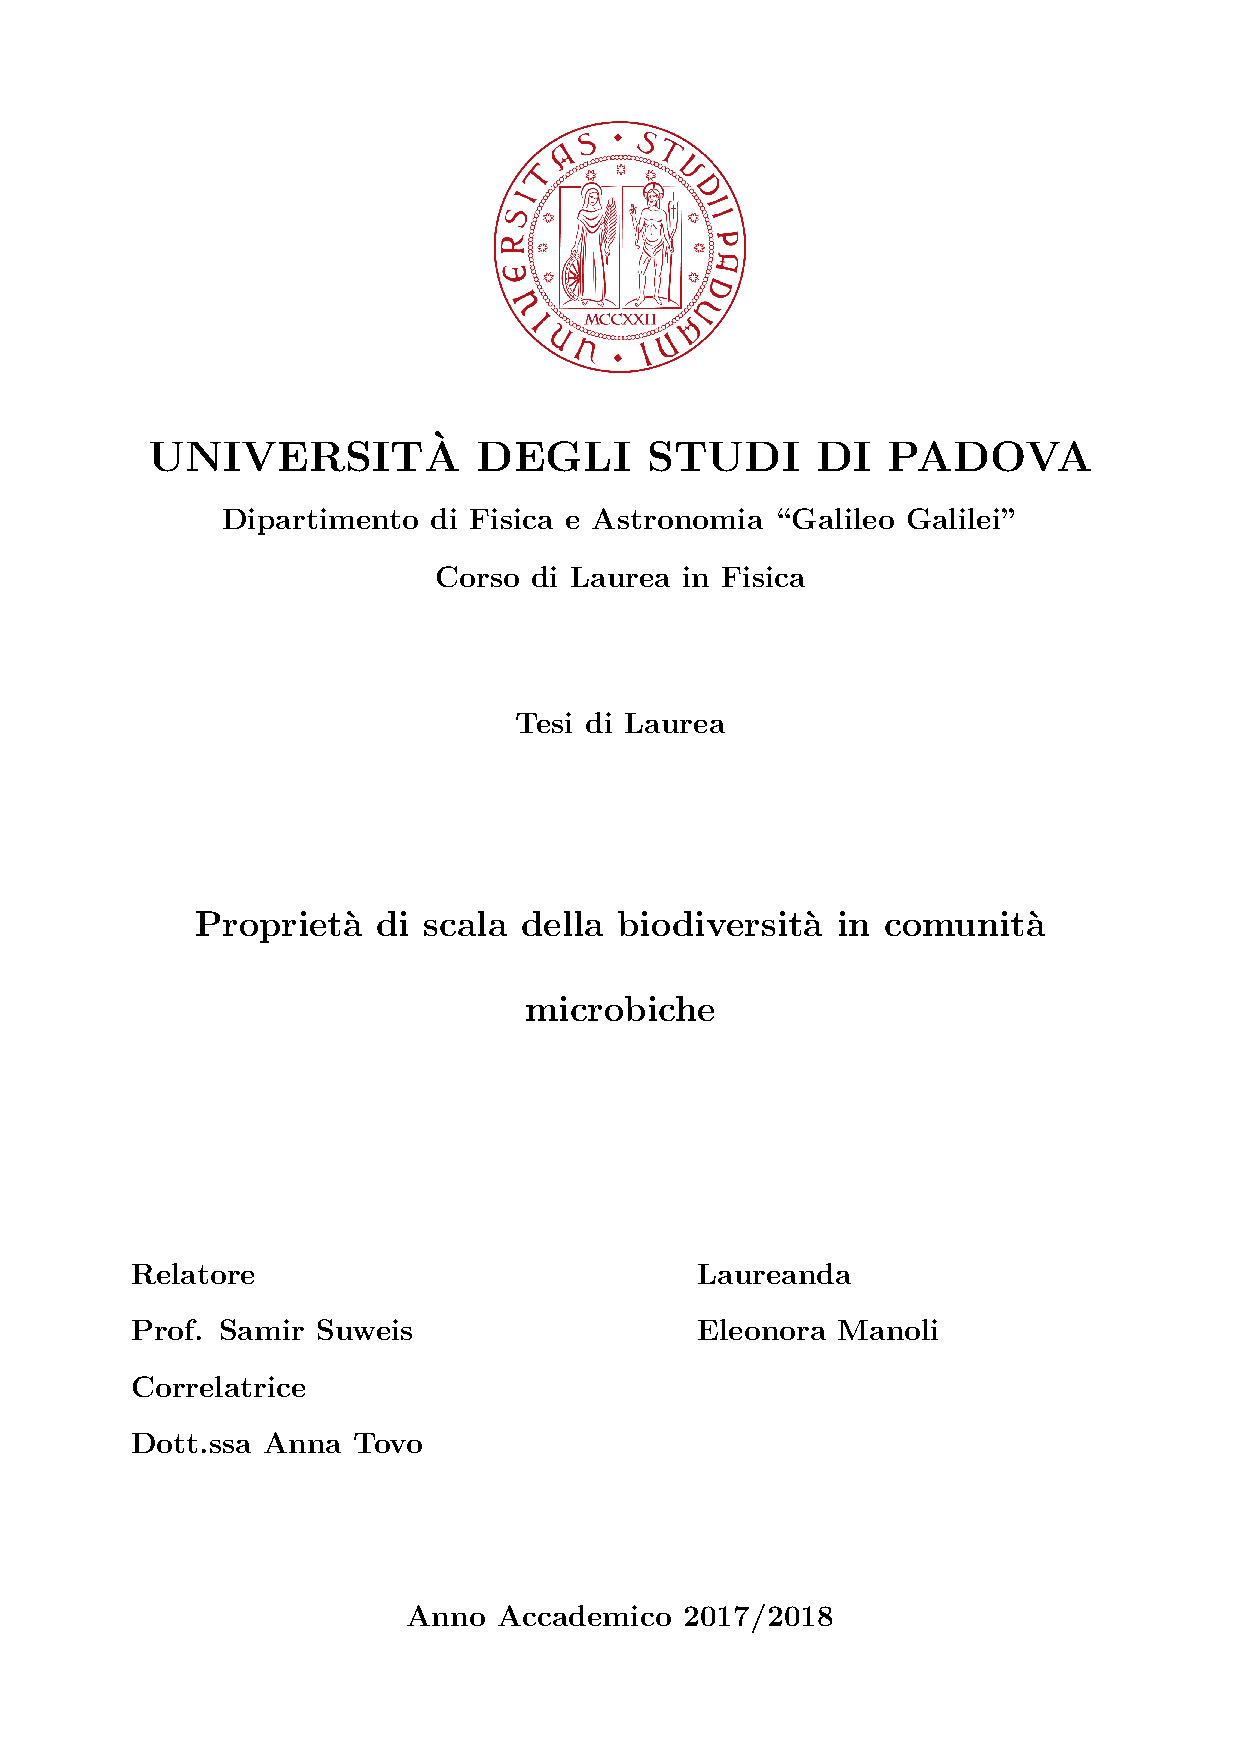
\includepdf{Frontespizio_Laurea.pdf}
\clearpage
\thispagestyle{empty}
\phantom{a}
%\maketitle
\chapter{Abstract}
 

% -------------------------------- TRACCIA GUIDA PER LA STESURA ------------------------------
%Il sommario � un breve riassunto dell'elaborato, orientativamente di circa 200 parole. In
%esso il laureando deve esporre concisamente:
%
%\begin{itemize}
%\item il problema che � stato considerato
%\item come il problema � stato risolto
%\item i principali risultati e il relativo significato.
%\end{itemize}
%
%Il sommario deve essere informativo e non una semplice lista di argomenti svolti; da una
%sua lettura, con una preparazione media sull'argomento, si dovrebbe capire se il lavoro �
%di interesse per chi si accinge a consultare la tesi.


In ecologia, un problema nella caratterizzazione della biodiversità di un ecosistema è quello di stimarla utilizzando solo campioni locali, i quali coprono solamente una minima percentuale dell'area su cui si estende il sistema in esame. In questa tesi, seguendo il lavoro presentato nell'articolo "Upscaling species richness and abundances in tropical forests"\cite{Tovoe1701438}, recentemente pubblicato su Science Advance, verranno presentati alcuni dei metodi più utilizzati per superare tale problema ponendo l'accento su come questi derivino naturalmente da principi primi alla base dei processi biologici. Un problema analogo si presenta anche nello studio delle comunità microbiche.\newline
Dopo aver testato l'affidabilità dei modelli in questo ambito, verranno applicati a dei dati presi dallo studio "Characterization of the gut microbiome using $16S$ or shotgun metagenomics"\cite{shotgun}.

\clearemptydoublepage

% Indice della tesi
\tableofcontents

%\mainmatter

\clearemptydoublepage

\mainmatter

%\chapter*{Introduzione}
\addcontentsline{toc}{chapter}{Introduzione}
Ogni volta che inviamo una e-mail, visitiamo un sito web o chattiamo con qualcuno, i nostri pacchetti attraversano vari router/server che possono controllare i dati inoltrati. Anche se i dati contenuti nei pacchetti sono crittografati, l'IP header rimane comunque visibile, ed � quindi possibile scoprire le identit� del mittente e del destinatario. Intercettando e analizzando i pacchetti, una spia pu� ottenere un numero considerevole di informazioni circa l'identit� dei soggetti della comunicazione, l'applicazione che li ha generati e talvolta il loro contenuto.
I sistemi di anonymous routing, come l'\emph{Onion Routing}\cite{tor}, nascono per garantire la segretezza nelle comunicazioni e l'anonimato delle parti coinvolte.

L'Onion routing � il pi� diffuso sistema di comunicazione anonimo a bassa latenza, permette web browsing, invio di e-mail, messaggistica istantanea e altri servizi. Esso si basa sulla rete \emph{Tor (The Onion Router)}, formata da un gruppo di volontari, che donano la propria banda per permettere agli utenti di aumentare la loro privacy e la loro sicurezza. La rete viene anche utilizzata come strumento per aggirare censure e blocchi imposti dagli ISP e, pi� in generale, il controllo delle comunicazioni da parte dei governi e dei regimi repressivi. Milioni di persone ogni giorno usano Tor per svolgere le loro attivit� quotidiane (come e-mail, Facebook, Twitter) senza il timore di essere monitorati. Per questo in alcuni paesi del mondo, come Cina, Iran, Kazakistan ecc. si tenta di arginare il pi� possibile la diffusione e l'utilizzo di Tor. In altri paesi, come gli Stati Uniti, viene usato dalla Marina Militare per svolgere operazioni di intelligence e dalle forze dell'ordine per controllare siti web, senza lasciare tracce di indirizzi IP governativi. Anche organizzazioni come Wikileaks utilizzano Tor per scambiare informazioni e tutelare i propri informatori. Attualmente, la rete conta circa 7000 router attivi e approssimativamente 2 milioni di client che si collegano ogni giorno \cite{tormetrics}.



%\emph{anonimato}, \emph{non linkabilit�}, \emph{inosservabilit�}.



%\cite{tor}, nascono per garantire segretezza nelle comunicazioni, in particolare cercando di raggiungere degli obiettivi fondamentali:
%\begin{description}
%\item \textbf{Anonimity}, definita come lo stato di non essere identificabili all'interno di un insieme di soggetti.
%\item \textbf{Unlinkability}.
%\item \textbf{Unobservability}.
%\end{description} 

%i client devono potersi scambiare messaggi in totale anonimato, questo significa che essi non devono essere identificabili all'interno di un insieme di soggetti.


%
%\lipsum[1-4]
%wikileaks

%Essa � costruita sopra ad internet...

%Perch� anonimato, blocco dei governi, cos � attacco dos


%non lascia traccia sui server, IP, vedi survey, gestita da volontari, %dati riguardanti utilizzo di tor, grafici

%\section{Perch\`e l'anonimato}

%\section{Blocco da parte dei governi}

\subsubsection{Attacchi DoS}
L'acronimo \emph{DoS}, abbreviazione di \emph{denial of service}, letteralmente negazione del servizio, indica una tipologia di attacchi informatici che mirano ad esaurire le risorse di un sistema, tipicamente un web server o un router, fino a renderlo non pi� in grado di fornire i propri servizi ai client. Esso non � un attacco caratteristico della rete Tor, dato che, attraverso varie tecniche, pu� essere effettuato contro qualsiasi sistema collegato ad Internet che offre servizi TCP. Quello che � possibile fare, per�, � sfruttare delle debolezze di progettazione del protocollo di Tor per condurre degli attacchi che in una normale rete TCP non sarebbero possibili. Come nei classici attacchi DoS, anche quelli che sfruttano le vulnerabilit� di Tor mirano al consumo di banda, di risorse computazionali o di memoria. Gli attacchi DoS sulle reti di anonimato possono essere suddivisi in due categorie: \emph{blanket blocking}, che blocca l'accesso all'intera rete senza attaccare in modo diretto alcun router, come ad esempio i blocchi imposti dai governi, oppure \emph{targeted attack}, ovvero attacchi con un obiettivo specifico, che tentano di portare nodi della rete offline. Portando offline i router portanti della rete, � possibile, probabilisticamente parlando, deanonimizzare servizi nascosti, scoprire l'identit� di due interlocutori o comunque causare un calo di prestazioni della rete che pu� indurre gli utenti ad utilizzare altri metodi di comunicazione meno sicuri di Tor. 



%Inoltre, molto spesso, vengono utilizzati per scoprire l'identit� di un server o per 

           
%\lipsum[1]

%\chapter{Introduzione}
%L'introduzione costituisce la prima parte dell'elaborato ed estende quanto contenuto nel
%sommario, orientando meglio la lettura. In essa vanno inserite le informazioni che stanno a
%monte, logicamente e cronologicamente, al lavoro svolto nella tesi. Si compone
%essenzialmente dei seguenti punti:
%\begin{itemize}
%\item spiegazione della natura del problema considerato
%\item descrizione dei contenuti reperibili in letteratura relativamente al problema in
%questione, corredata da esaurienti citazioni bibliografiche
%\item scopo del lavoro
%\item indicazione dei metodi di soluzione del problema
%\item elenco schematico del contenuto dei vari capitoli.
%\end{itemize}
%
%\clearemptydoublepage

\chapter*{Introduzione}
\addcontentsline{toc}{chapter}{Introduzione}
Ogni volta che inviamo una e-mail, visitiamo un sito web o chattiamo con qualcuno, i nostri pacchetti attraversano vari router/server che possono controllare i dati inoltrati. Anche se i dati contenuti nei pacchetti sono crittografati, l'IP header rimane comunque visibile, ed � quindi possibile scoprire le identit� del mittente e del destinatario. Intercettando e analizzando i pacchetti, una spia pu� ottenere un numero considerevole di informazioni circa l'identit� dei soggetti della comunicazione, l'applicazione che li ha generati e talvolta il loro contenuto.
I sistemi di anonymous routing, come l'\emph{Onion Routing}\cite{tor}, nascono per garantire la segretezza nelle comunicazioni e l'anonimato delle parti coinvolte.

L'Onion routing � il pi� diffuso sistema di comunicazione anonimo a bassa latenza, permette web browsing, invio di e-mail, messaggistica istantanea e altri servizi. Esso si basa sulla rete \emph{Tor (The Onion Router)}, formata da un gruppo di volontari, che donano la propria banda per permettere agli utenti di aumentare la loro privacy e la loro sicurezza. La rete viene anche utilizzata come strumento per aggirare censure e blocchi imposti dagli ISP e, pi� in generale, il controllo delle comunicazioni da parte dei governi e dei regimi repressivi. Milioni di persone ogni giorno usano Tor per svolgere le loro attivit� quotidiane (come e-mail, Facebook, Twitter) senza il timore di essere monitorati. Per questo in alcuni paesi del mondo, come Cina, Iran, Kazakistan ecc. si tenta di arginare il pi� possibile la diffusione e l'utilizzo di Tor. In altri paesi, come gli Stati Uniti, viene usato dalla Marina Militare per svolgere operazioni di intelligence e dalle forze dell'ordine per controllare siti web, senza lasciare tracce di indirizzi IP governativi. Anche organizzazioni come Wikileaks utilizzano Tor per scambiare informazioni e tutelare i propri informatori. Attualmente, la rete conta circa 7000 router attivi e approssimativamente 2 milioni di client che si collegano ogni giorno \cite{tormetrics}.



%\emph{anonimato}, \emph{non linkabilit�}, \emph{inosservabilit�}.



%\cite{tor}, nascono per garantire segretezza nelle comunicazioni, in particolare cercando di raggiungere degli obiettivi fondamentali:
%\begin{description}
%\item \textbf{Anonimity}, definita come lo stato di non essere identificabili all'interno di un insieme di soggetti.
%\item \textbf{Unlinkability}.
%\item \textbf{Unobservability}.
%\end{description} 

%i client devono potersi scambiare messaggi in totale anonimato, questo significa che essi non devono essere identificabili all'interno di un insieme di soggetti.


%
%\lipsum[1-4]
%wikileaks

%Essa � costruita sopra ad internet...

%Perch� anonimato, blocco dei governi, cos � attacco dos


%non lascia traccia sui server, IP, vedi survey, gestita da volontari, %dati riguardanti utilizzo di tor, grafici

%\section{Perch\`e l'anonimato}

%\section{Blocco da parte dei governi}

\subsubsection{Attacchi DoS}
L'acronimo \emph{DoS}, abbreviazione di \emph{denial of service}, letteralmente negazione del servizio, indica una tipologia di attacchi informatici che mirano ad esaurire le risorse di un sistema, tipicamente un web server o un router, fino a renderlo non pi� in grado di fornire i propri servizi ai client. Esso non � un attacco caratteristico della rete Tor, dato che, attraverso varie tecniche, pu� essere effettuato contro qualsiasi sistema collegato ad Internet che offre servizi TCP. Quello che � possibile fare, per�, � sfruttare delle debolezze di progettazione del protocollo di Tor per condurre degli attacchi che in una normale rete TCP non sarebbero possibili. Come nei classici attacchi DoS, anche quelli che sfruttano le vulnerabilit� di Tor mirano al consumo di banda, di risorse computazionali o di memoria. Gli attacchi DoS sulle reti di anonimato possono essere suddivisi in due categorie: \emph{blanket blocking}, che blocca l'accesso all'intera rete senza attaccare in modo diretto alcun router, come ad esempio i blocchi imposti dai governi, oppure \emph{targeted attack}, ovvero attacchi con un obiettivo specifico, che tentano di portare nodi della rete offline. Portando offline i router portanti della rete, � possibile, probabilisticamente parlando, deanonimizzare servizi nascosti, scoprire l'identit� di due interlocutori o comunque causare un calo di prestazioni della rete che pu� indurre gli utenti ad utilizzare altri metodi di comunicazione meno sicuri di Tor. 



%Inoltre, molto spesso, vengono utilizzati per scoprire l'identit� di un server o per 

           
%\lipsum[1]

%\chapter{Introduzione}
%L'introduzione costituisce la prima parte dell'elaborato ed estende quanto contenuto nel
%sommario, orientando meglio la lettura. In essa vanno inserite le informazioni che stanno a
%monte, logicamente e cronologicamente, al lavoro svolto nella tesi. Si compone
%essenzialmente dei seguenti punti:
%\begin{itemize}
%\item spiegazione della natura del problema considerato
%\item descrizione dei contenuti reperibili in letteratura relativamente al problema in
%questione, corredata da esaurienti citazioni bibliografiche
%\item scopo del lavoro
%\item indicazione dei metodi di soluzione del problema
%\item elenco schematico del contenuto dei vari capitoli.
%\end{itemize}

\clearemptydoublepage

\chapter{Modelli di campionamento e analisi}







%Ricordiamo che, in questo contesto, i dati che abbiamo a disposizione per prevedere la biodiversità degli ecosistemi sono dati di abbondanza: per una certa frazione di area vengono registrate le specie osservate e il numero di individui per specie presenti nel campione ottenendo così un vettore di abbondanze.
%Dunque vengono raccolte solo le frequenze con cui si presentano le varie specie e queste ultime sono sufficienti per stimare la ricchezza delle specie. 
%In questo schema di campionamento la misura del campione \emph{n} (il numero di individui osservati nell'esperimento) è una variabile casuale e può assumere qualsiasi valore intero.\\


La ricchezza delle specie è la misura più intuitiva e più frequentemente usata per caratterizzare la diversità di un dato ecosistema. \\
La ricchezza di specie dipende però fortemente dal metodo di campionamento e dalla completezza del campione. Il modo tipico di censimento di una comunità ecologica porta ad avere principalmente due tipi di dati: dati di abbondanza e dati di incidenza\cite{doi:ChaoChiu2016}\cite{presabs}.\\
Per fissare la notazione: consideriamo una comunità costituita da N individui appartenenti a $S$ specie distinte. Sia $N_\emph{i}$ il numero di individui della \emph{i}-esima specie con \emph{i}=1,2,...,S, $N_\emph{i}>0$ e $N=\sum_{n=1}^S N_\emph{i}$.
L'abbondanza relativa della specie \emph{i}-esima è $p_\emph{i}=N_\emph{i}/N$, dunque $\sum_{n=1}^S p_\emph{i}=1$. Qui N, S, $N_\emph{i}$ e $p_\emph{i}$ rappresentano i valori veri, ma sconosciuti, dei parametri fondamentali dell'insieme in esame.\\

\subsubsection{Dati di abbondanza}
In molti studi biologici o ecologici solitamente gli individui vengono osservati in un dato momento e vengono classificati in base alla specie di appartenenza. Si prenda ad esempio un campione di \emph{n} individui dall'insieme in esame e si ipotizzi di osservare un totale di $S^*$ specie: questo è il \emph{campione di riferimento}. Questo tipo di data-set può essere ottenuto usando due schemi di campionamento differenti:
\begin{enumerate}
    \item \emph{campionamento di tipo discreto} in cui l'unità campionaria è un individuo. Ad esempio, si campiona un numero fissato $N^*$ di individui in una certa area. Qui la grandezza del campione \emph{n} è fissata e ogni specie può essere rappresentata al massimo da $N^*$ individui;
    
    \item \emph{campionamento di tipo continuo} nel quale il campione viene quantificato misurando su scale continue come tempo, area o volume d'acqua.
    Si fissa, per esempio, una certa area da studiare o un certo periodo di tempo nel quale analizzare il sito in esame. Con questo protocollo di campionamento il numero di individui osservati è una variabile casuale e ogni specie può essere rappresentata da un numero qualsiasi di individui.
\end{enumerate}

\subsubsection{Dati di incidenza}
In alcune indagini le unità di campionamento non sono gli individui, ma porzioni di area o periodi di tempo: queste vengono campionate casualmente e indipendentemente. Ad esempio un'area di interesse può essere divisa in un certo numero di celle approssimativamente della stessa sotto-area e, una volta selezionate casualmente alcune di queste, l'indagine viene condotta solo su di esse.\\
A volte risulta impossibile contare esattamente il numero di individui per ogni specie che appaiono in un campione (ad esempio per microrganismi, invertebrati o piante) e quindi viene registrata solo la loro incidenza (presenza o assenza) nel campione. Dunque le stime si basano su degli insiemi di unità di campionamento in cui è registrata solo la presenza o assenza di una certa specie in un dato campione invece che la sua abbondanza.
\\ \\
Avendo a disposizione questo tipo di dati si possono seguire due approcci per stimare la diversità del campione: quello parametrico e quello non parametrico.
In questo lavoro useremo dati di abbondanza ottenuti con campionamento continuo, infatti consideriamo una frazione \emph{a} di un'area $A$ nella quale sono stati registrati il numero di individui presenti con relativa specie di appartenenza. D'ora in poi ci occuperemo solo di questo caso particolare.

\subsubsection{Modelli parametrici e non parametrici}
Negli approcci parametrici che analizzeremo si assume che la distribuzione dell'abbondanza delle specie abbia una certa forma funzionale, governata da dei parametri. Facendo il fit della curva dell'abbondanza relativa delle specie dei dati osservati si ottengono i valori dei parametri che, secondo le caratteristiche e le proprietà della distribuzione ipotizzata, permettono di dedurre le informazioni sulla diversità del sistema osservato.\newline
Negli approcci non parametrici, invece, non si fanno assunzioni sulla distribuzione sottostante alla curva dell'abbondanza delle specie. L'intuizione e concetto base su cui si fondano i metodi di stima non parametrici è che le specie dominanti, cioè quelle a cui appartengono un elevato numero di individui, non danno alcuna informazione sulla ricchezza delle specie inosservate, mentre le specie rare, contengono quasi tutte le informazioni sulla biodiversità. Dunque, la maggior parte degli stimatori non parametrici si basa sulle frequenze di apparizione di basso ordine, specialmente sul numero di \emph{singletons} e \emph{doubletons}, cioè sul numero specie che vengono registrate contenere uno o due individui.


\clearemptydoublepage

\chapter{Derivazione delle distribuzioni binomiale negativa e logaritmica}
Nel modello parametrico analizzato in questo lavoro, assumeremo che la SAD sia ben descritta da una binomiale negativa.
Prima di entrare nel merito dei modelli per la stima del numero di specie, vediamo come si può ricavare tale distribuzione (come anche la distribuzione logaritmica, molto utilizzata in ecologia), modellando la dinamica stocastica dell'abbondanza delle specie attraverso la così detta \emph{birth-death master equation}\cite{2016AzaeleSuweis}.\\
Entrambe le distribuzioni (logaritmica e binomiale negativa) possono essere derivate da processi ecologici fondamentali quali appunto nascita, morte e migrazione. 

Sia $\emph{P}_{\emph{n,s}}(t)$ la probabilità che ad un certo tempo $t$, la specie \emph{s} abbia esattamente \emph{n} individui, con $\emph{s}\in\left \{ 1,...,S \right \}$. Assumiamo che la dinamica della popolazione di ogni specie $s=1,2,...,S$ con popolazione $n$ sia governata dai rates di nascita e di morte, rispettivamente, $\emph{b}_\emph{{n,s}}$ e $\emph{d}_\emph{{n,s}}$.
L'equazione che regola l'evoluzione di $\emph{P}_{\emph{n,s}}(t)$ per $\emph{n}\ge0$ sarà quindi:
\begin{equation}
\frac{\partial\emph{P}_{\emph{n,s}}(t)}{\partial\emph{t}}=
\emph{P}_{\emph{n-1,s}}(t)\emph{b}_\emph{{n-1,s}}+\emph{P}_{\emph{n+1,s}}(t)\emph{d}_\emph{{n+1,s}}-\emph{P}_{\emph{n,s}}(t)\emph{b}_\emph{{n,s}}-\emph{P}_{\emph{n,s}}(t)\emph{d}_\emph{{n,s}}.
\label{eq:master}
\end{equation}
In questo lavoro, per evitare che \emph{n} sia negativo, imponiamo delle condizioni al contorno riflettenti: $\emph{b}_\emph{{-1,s}}=\emph{d}_\emph{{0,s}}=0$. %la (\ref{eq:master}) è valida anche per $\emph{n}=0$ e \emph{n=1}. 
Si trova che per $\emph{n}>0$ la soluzione stazionaria è:
\begin{equation}
\emph{P}_{\emph{n,s}}=P_{0,\emph{s}}\prod_{i=0}^{n-1}\frac{\emph{b}_\emph{{i,s}}}{\emph{d}_\emph{{i+1,s}}}
\label{eq:steadystate}
\end{equation}
dove il termine $P_{0,\emph{s}}$ è il fattore di normalizzazione che può essere trovato imponendo la condizione $\sum_{n=1}^\infty \emph{P}_{\emph{n,s}}=1.$ Notiamo che la somma inizia da \emph{n}=1 in quanto non si considerano specie con abbondanza nulla.\\



\section{Distribuzione binomiale negativa}
Ipotizziamo che tutti gli individui, siano essi appartenenti a specie rare o comuni, abbiano la stessa probabilità di morire, sopravvivere e riprodursi. In questo caso i tassi di nascita e morte pro capite non dipendono dal numero di individui \emph{n} appartenenti alla specie.
Definiamo quindi $\emph{b}_\emph{{n,s}}$ come:
\begin{equation}
\emph{b}_\emph{n,s}=\emph{b}_\emph{s}(n+\emph{r}_\emph{s}),
\label{eq:birthNB}
\end{equation}
dove $\emph{r}_\emph{s}$ è un parametro che tiene conto di eventi di immigrazione o di interazioni intraspecifiche.\newline
Analogamente definiamo $\emph{d}_\emph{n,s}$: 
\begin{equation}
\emph{d}_\emph{n,s}=\emph{d}_\emph{s}\emph{n}.
\label{eq:deathNB}
\end{equation}

Sostituendo questi ultimi termini nella (\ref{eq:steadystate}) e denotando con $\xi_\emph{s}=\emph{b}_\emph{s}/\emph{d}_\emph{s}$, si ottiene:
$$
\emph{P}_\emph{n,s}=P_\emph{0,s}\binom{n+\emph{r}_\emph{s}-1}{n}\xi_\emph{s}^n.
$$
La costante di normalizzazione può essere calcolata imponendo:
$$
1=\sum_{n=1}^\infty \emph{P}_{\emph{n,s}}=P_\emph{0,s}\sum_{n=1}^\infty\binom{n+\emph{r}_\emph{s}-1}{n}\xi_\emph{s}^n=P_\emph{0,s}[1-(1-\xi_\emph{s})^{\emph{r}_\emph{s}}](1-\xi_\emph{s})^{-\emph{r}_\emph{s}}.
$$
Dunque la probabilità che una specie \emph{s} abbia \emph{n} individui all'equilibrio è data da una binomiale negativa di parametri $(\emph{r}_\emph{s}, \xi_\emph{s})$ e normalizzata per abbondanze non nulle ($n\ge 1$):
\begin{equation}
\emph{P}_\emph{n,s}^{\emph{NB}}=\frac{1}{1-(1-\xi_\emph{s})^{\emph{r}_\emph{s}}}\binom{n+\emph{r}_\emph{s}-1}{n}\xi_\emph{s}^n(1-\xi_\emph{s})^{\emph{r}_\emph{s}}.
\label{eq:NBprobability}
\end{equation}
Sotto l'ipotesi della teoria neutrale secondo la quale le specie sono considerate demograficamente equivalenti, possiamo rimuovere l'indice \emph{s} di specie dall'equazione sopra, ottenendo così una SAD per l'ecosistema in esame. Notiamo che quindi in questo framework, la dinamica della popolazione della specie è determinata puramente da processi demografici random (nascita, morte e migrazione) e ogni specie rappresenta una diversa realizzazione dello stesso processo stocastico.

\section{Distribuzione logaritmica di Fisher}
Notiamo che, scegliendo in modo diverso il termine $\emph{b}_\emph{n,s}$, si può ottenere sempre attraverso la \emph{birth-death master equation} (\ref{eq:master}), un'altra importante distribuzione: la distribuzione logaritmica di Fisher.
Consideriamo ora nella dinamica della comunità ecologica anche il fenomeno di speciazione (cioè l'entrata di nuove specie nel sistema dovute a mutazioni, invece che a migrazione da comunità esterne). La speciazione avverrà con un rate molto piccolo $\nu$, e si avrà:
\begin{equation}
    \emph{b}_\emph{n,s}=\emph{b}_\emph{s}n+\delta_\emph{n,0}\nu.
\label{eq:birthlog}
\end{equation}
Aggiungendo la condizione al contorno riflettente $\emph{b}_\emph{0,s}=\nu$ si ha quindi che il tasso di nascita tiene conto della riproduzione e della speciazione. In particolare, il parametro $\nu$ assicura che, se le specie si estinguono, la comunità rimane sempre popolata da un individuo.
Dunque sostituendo la (\ref{eq:deathNB}) e la (\ref{eq:birthlog}) nella (\ref{eq:steadystate}) e definendo $\emph{x}_\emph{s}=\emph{b}_\emph{s}/\emph{d}_\emph{s}$, si trova la seguente soluzione stazionaria:
\begin{equation}
    \emph{P}_\emph{n,s}=P_\emph{0,s}\frac{\nu}{\emph{b}_\emph{s}}\frac{\emph{x}_\emph{s}^{\emph{n}}}{\emph{n}}.
\end{equation}
La costante di normalizzazione $P_\emph{0,s}$ si determina imponendo:
$$
1=\sum_{n=1}^\infty \emph{P}_{\emph{n,s}}=P_\emph{0,s}\frac{\nu}{\emph{b}_\emph{s}}\sum_{n=0}^\infty\frac{\emph{x}_\emph{s}^{\emph{n}}}{\emph{n}}=P_\emph{0,s}\frac{\nu}{\emph{b}_\emph{s}}[-\log(1-\emph{x}_\emph{s})].
$$
Dunque abbiamo:
\begin{equation}
    \emph{P}_\emph{n,s}^{\emph{LS}}=-\frac{1}{\log(1-\emph{x}_\emph{s})}\frac{\emph{x}_\emph{s}^{\emph{n}}}{\emph{n}}.
\label{eq:fisherdist}
\end{equation}
Anche in questo caso assumiamo che le specie siano equivalenti e possiamo dunque omettere l'indice \emph{s}.

\subsection{La distribuzione di Fisher come caso particolare della binomiale negativa}
Osserviamo che la distribuzione binomiale negativa converge ad una distribuzione logaritmica nel limite di \emph{r} che tende a zero:
\begin{equation}
    \lim_{\emph{r} \to 0}\emph{P}_\emph{n}^{\emph{NB}}= \lim_{\emph{r}\to0}\frac{(1-\xi)^{\emph{r}}}{1-(1-\xi)^{\emph{r}}}\binom{n+\emph{r}-1}{n}\xi^n=\frac{\xi^n}{-n\ln(1-\xi)},
\label{eq:convergence}
\end{equation}
dove si è usato il fatto che:
$$
\binom{n+\emph{r}-1}{n}=\frac{\Gamma(\emph{n}+\emph{r})}{\Gamma(\emph{n+1})\Gamma(\emph{r})} \approx\frac{\emph{r}}{\emph{n}},
$$
per $\emph{r}\approx 0$.\\
Notiamo dunque che la (\ref{eq:convergence}) coincide con la (\ref{eq:fisherdist}) ponendo  $\emph{x}=\xi$.


%\section{Protocolli crittografici}
%HTTPS, TLS, Diffie-Hellman, SHA-1
% ---- ELEMENTI UTILI E GIA' PRONTI! ----
%Secondo capitolo della tesi. Esempio di citazione doppia \cite{Munoz-Lipo,Vas}.

%Esempio di figura in \figurename\ \ref{FIG:LogoUniPD}.
%
%\begin{figure}[!htbp]
%\centering
%
\includegraphics[width=0.25\textwidth]{./figure//LogoUniPD}
%\caption{Esempio di figura.}
%\label{FIG:LogoUniPD}
%\end{figure}
%
%Esempio di tabella in \tablename\ \ref{TAB:Esempio}.
%
%\begin{table}[!htbp]
%\centering
%\renewcommand{\arraystretch}{1.3}
%\caption{Esempio di tabella.}
%\begin{tabular}{cc}
%\hline
%Nome & Valore \\
%\hline
%a & 1 \\
%b & 2 \\
%c & 3 \\
%d & 4 \\
%e & 5 \\
%f & 6 \\
%\hline
%\end{tabular}
%\label{TAB:Esempio}
%\end{table}

\clearemptydoublepage

\chapter{Metodi di upscaling}
Con il termine \emph{upscaling} si intende inferire informazioni "a scala più grande": in questo contesto significa predire il numero di specie presenti a scale più grandi di quelle che, per motivi pratici, possono essere indagate sperimentalmente e di cui si hanno dunque dati certi.\\
In questa sezione vediamo in dettaglio come è possibile ricostruire la biodiversità di un intero ecosistema a partire da un campione ridotto di SAD, occupandoci del caso in cui ad essere studiata è una frazione dell'area totale del sistema in esame.\\
Analizzeremo prima due metodi parametrici, quello della binomiale negativa e della distribuzione logaritmica di Fisher \cite{Tovoe1701438}, e poi un metodo non parametrico, quello dello stimatore di $Chao_\emph{wor}$\cite{Chaowor}.

\subsubsection{Ipotesi sul metodo di upscaling}
Nella nostra analisi assumiamo che la probabilità \emph{p} che un individuo si trovi all'interno di una zona \emph{a} contenuta in una regione \emph{A} sia proporzionale all'area della zona stessa: \emph{p}=\emph{a}/\emph{A}. Ci riferiamo a quest'ipotesi con il nome di \emph{ipotesi di campo medio}. Una conseguenza di ciò è che campionare una frazione \emph{p} di un'area \emph{A} in cui ogni individuo viene catalogato in una lista in base alla specie di appartenenza è equivalente a campionare la stessa frazione \emph{p} degli individui sulla lista. Questa è l'unica procedura imparziale che può essere adottata quando non si hanno informazioni né sulle posizioni degli individui né sulle correlazioni spaziali. Per ritenere quest'ipotesi soddisfatta bisogna verificare che la regione in esame non presenti forti disomogeneità e anisotropie, altrimenti alcune specie tenderebbero ad abitare habitat specifici all'interno della regione e dunque l'assunzione di avere una distribuzione spazialmente omogenea degli individui non sarebbe più valida.\\
%(spiegare che il modello nasce in ambito ecologico)\\
%(come viene fatto il campionamento)\\
%(parlare in generale, numero di singleton, specie rare)\\
%(metodo di Chao??)\\
\\

\section{Metodo della binomiale negativa}
%Il quadro analitico all'interno del quale si svolge questo lavoro è bastato sui seguenti passaggi:
%\begin{itemize}
  %  \item Campionare una frazione $\emph{p}^*$ dell'intera foresta e ottenere il vettore delle abbondanze delle $S^*$ specie campionate, $\emph{n}_{\emph{p}^*}={\emph{n}_1,\emph{n}_2,...,\emph{n}_{S^*}}$
  % \item Usare una combinazione lineare di binomiali negative con lo stesso $\hat \xi_{\emph{p}^*}$ e diversi valori di \emph{r} per fittare la SAD sperimentale al desiderato grado di accuratezza.
%\end{itemize}
%Di seguito analizzeremo in dettaglio le proprietà e i passaggi che ci permettono di ottenere le informazioni desiderate.\\
Quando facciamo\emph{ upscaling} siamo interessati alla SAD ed al numero totale di specie presenti a scala globale, cioè in tutta l'area \emph{A} dell'ecosistema in esame.
Denotiamo con $P(\emph{n}|1)$ la probabilità che una specie abbia esattamente \emph{n} individui a scala globale (con il numero 1 si intende l'intero ecosistema), anche nota come \emph{abbondanza relativa delle specie} (RSA).
Notiamo che P(\emph{n}|1) deve essere definita solamente per $\emph{n}\ge1$ poiché per poter osservate una data specie questa deve essere popolata da almeno un individuo.\newline
In questo metodo di \emph{upscaling} si ipotizza che la SAD segua una distribuzione binomiale negativa $\mathcal{P}(\emph{n}|\emph{r},\xi)$ di parametri (\emph{r},$\xi$):
\\ 
\begin{equation}
 P(\emph{n}|1)=\emph{c}(\emph{r},\xi)\mathcal{P}(\emph{n}|\emph{r},\xi)
 \label{eq:NBfunctform}
\end{equation}
con 
\begin{equation}
    \mathcal{P}(\emph{n}|\emph{r},\xi)=\binom{n+\emph{r}-1}{n}\xi^n(1-\xi)^{\emph{r}}     
\end{equation}
e
\begin{equation}
     \emph{c}(\emph{r},\xi)=\frac{1}{1-(1-\xi)^{\emph{r}}}
\end{equation}
\\ 
dove \emph{c} è la costante di normalizzazione.
Quest'ultima è stata calcolata imponendo \newline  $\sum_{\emph{n}=1}^\infty P(\emph{n}|1)=1$, dove la somma parte da 1 poiché  non si possono osservare specie con abbondanza nulla.
Notiamo che invece $\mathcal{P}(\emph{n}|\emph{r},\xi)$è normalizzata per $\emph{n}\ge0$: questo perché nei campioni esiste una probabilità non nulla di che una specie presente nell'intero ecosistema abbia \emph{n}=0 individui. Dunque in questo modo si tiene conto del numero di specie mancanti nei campioni.\\
Consideriamo ora un campione di area \emph{a} e definiamo \emph{p}=\emph{a}/\emph{A} la scala del campione, cioè la frazione di ecosistema osservato.
Come primo passaggio calcoliamo la RSA del campione assumendo che quest'ultima non sia influenzata da correlazioni spaziali. Quest'ipotesi è ben soddisfatta ed è stata verificata usando dati di foreste generati \emph{in silico} a vari gradi di correlazione spaziale\cite{Tovoe1701438}.\\
Sotto queste ipotesi la probabilità che una specie presenti \emph{k} individui in un'area \emph{a=pA}, condizionata dal fatto che presenta \emph{n} individui nella regione totale \emph{A} è data dalla distribuzione binomiale:
\\ 
\begin{equation}
\mathcal{P}_\emph{binom}(\emph{k}|\emph{n},\emph{p})=\begin{cases} \binom{\emph{n}}{\emph{k}}\emph{p}^\emph{k}(1-\emph{p})^{\emph{n-k}} & \mbox{se }\emph{k}=0,...,\emph{n} \\ 0 & \mbox{se }\mbox{\emph{k>n}}
\end{cases}
\end{equation}
\\ 

Infatti, in assenza di correlazioni spaziali, la probabilità che uno degli individui di una specie si trovi in una regione di area \emph{a} è esattamente \emph{p}.

Mostriamo ora un risultato chiave per il metodo di upscaling:
\subsection{Proprietà di invarianza per forma 
della distribuzione binomiale negativa}
Sia $ P(\emph{n}|1)=\emph{c}(\emph{r},\xi)\mathcal{P}(\emph{n}|\emph{r},\xi) $ la RSA dell'ecosistema a scala globale e denotiamo con $\mathcal{P}(\emph{k}|\emph{n},\emph{p})$ la probabilità che una specie abbia abbondanza \emph{k} alla scala \emph{p}$\in$(0,1) condizionata dal fatto che alla scala globale \emph{A} sono presenti \emph{n} individui di quella specie.
Se $\mathcal{P}(\emph{k}|\emph{n,p})=\mathcal{P}_\emph{binom}(\emph{k}|\emph{n},\emph{p})$ segue una distribuzione binomiale, allora la RSA $\mathcal{P}_\emph{sub}(\emph{k}|\emph{p})$ alla scala di campionamento \emph{p} è ancora una binomiale negativa per $\emph{k}\ge1$ con il parametro $\xi$ riscalato e lo stesso \emph{r}:
\\ \\
\begin{equation}
    \mathcal{P}_\emph{sub}(\emph{k}|\emph{p})=\begin{cases} \emph{c}(\emph{r},\xi)\mathcal{P}(\emph{k}|\emph{r},\hat \xi_\emph{p}), & \mbox{ }\emph{k}\ge1 \\ 1-\emph{c}(\emph{r},\xi)/\emph{c}(\emph{r},\hat\xi_{\emph{p}}), & \mbox{ }\mbox{\emph{k=0}}
    \end{cases}
\label{eq:RSAbinom}
\end{equation}

con 
\begin{equation}
    \hat\xi_{\emph{p}}=\frac{\emph{p}\xi}{1-\xi(1-\emph{p})}.
\label{eq:NBparametersub}
\end{equation}
Infatti la probabilità $P_\mathcal{sub}(\emph{k}|\emph{p})$ di trovare una specie popolata da $\emph{k} \ge 0$ individui nel campione di area \emph{a}=\emph{p}\emph{A} è:
%\begin{proof}

\begin{equation}
   % \begin{aligned}
  %  A & = B + C\\
  %    & = D + E + F\\
   %   & = G
  %\end{aligned}
  \begin{aligned}
   \emph{k}\ge 1: \mathcal{P}_\emph{sub}(\emph{k}|\emph{p}) & = \sum_{\emph{n}\ge \emph{k}}\mathcal{P}_\emph{binom}(\emph{k}|\emph{n},\emph{p})P(\emph{n}|1)\\
      & = \sum_{\emph{n}\ge \emph{k}} \binom{\emph{n}}{\emph{k}}\emph{p}^\emph{k}(1-p)^{\emph{n}-\emph{k}} \cdot\emph{c}(\emph{r},\xi) \binom{\emph{n}+\emph{r}-1}{\emph{n}}\xi ^ \emph{n}(1-\xi)^\emph{r}\\
      & =\emph{c}(\emph{r},\xi)\binom{\emph{k}+\emph{r}-1}{\emph{k}}\left( \frac{\emph{p}\xi}{1-\xi(1-\emph{p})} \right)^\emph{k}\left( \frac{1-\xi}{1-\xi(1-\emph{p})} \right)^\emph{r} \\
      & = \emph{c}(\emph{r},\xi)\binom{\emph{k}+\emph{r}-1}{\emph{k}} \hat \xi_\emph{p}^\emph{k}(1-\hat \xi_\emph{p})^\emph{r} = \emph{c}(\emph{r},\xi)\cdot \emph{P}(\emph{k}|\emph{r},\hat \xi_\emph{p})
  \end{aligned}
\end{equation}

dove abbiamo usato la (\ref{eq:NBparametersub}) per $\hat \xi_\emph{p}$ per la penultima uguaglianza, e

 \begin{equation}
     \begin{aligned}
         \emph{k}=0: \mathcal{P}_\emph{sub}(0|\emph{p}) & =1-\sum_{\emph{n}\ge\emph{1}}\mathcal{P}_\emph{sub}(\emph{k}|\emph{p}) \\
         &=1-\sum_{\emph{n}=1}^\infty \emph{c}(\emph{r},\xi)\cdot \binom{\emph{k}+\emph{r}-1}{\emph{k}}\hat \xi_\emph{p}^\emph{k}(1-\hat \xi_\emph{p})^\emph{r}\\
         &=1-\emph{c}(\emph{r},\xi)\cdot \sum_{\emph{k}=1}^\infty \mathcal{P}(\emph{k}|\emph{r},\hat \xi _\emph{p})=1-\frac{\emph{c}(\emph{r},\xi)}{\emph{c}(\emph{r}, \hat \xi_\emph{p})}.
     \end{aligned}
 \end{equation}
 
%\end{proof}
 
\subsection{Il numero di specie a scala globale}
Ricordiamo che questo metodo fa uso solamente delle informazioni che si possono ottenere da un campione ad una certa scala $p^*$, infatti noi abbiamo informazioni solo sulle abbondanze delle $S^*\le S$ specie presenti nel campione esaminato. Denotando il numero di specie di abbondanza \emph{k} alla scala $p^*$ con $S^*(\emph{k})$, otteniamo, per $\emph{k}\ge 1$:

\begin{equation}
    \frac{S^*(\emph{k})}{S^*}\equiv P(\emph{k}|\emph{p}^*)=\frac{\mathcal{P}_\emph{sub}(\emph{k}|\emph{p}^*)}{\sum_{k^{'} \ge 1}^{} \mathcal{P}_\emph{sub}(\emph{k}^{'}|\emph{p}^{*})}
    =\frac{\mathcal{P}(\emph{k}|\emph{r},\hat\xi_{\emph{p}^*})}{\sum_{k^{'} \ge 1}^{} \mathcal{P}(\emph{k}^{'}|\emph{r},\hat \xi_{\emph{p}^*})}
    =\emph{c}(\emph{r},\hat\xi_{\emph{p}^*})\mathcal{P}(\emph{k}|\emph{r},\hat \xi_{\emph{p}^*})
    \label{eq:SstarRSA}
\end{equation}

che, dalla (\ref{eq:NBfunctform}), è una binomiale negativa normalizzata per $\emph{k}\ge 1$, mentre $\mathcal{P}(\emph{k}|\emph{r},\hat \xi_{\emph{p}^*})$ è normalizzata per $\emph{k}\ge 0$.
Per quanto detto sopra otteniamo dunque il seguente risultato: partendo da una distribuzione binomiale negativa per la RSA a scala globale, anche la RSA a scala ridotta risulta distribuita secondo una binomiale negativa di parametri lo stesso \emph{r} e $\hat \xi_\emph{p}^*$ riscalato.
Una RSA avente la proprietà di avere la stessa forma funzionale a scale differenti è detta essere \emph{invariante per forma}.

Fittando la RSA dei dati alla scala $\emph{p}^*$ possiamo dunque trovare i parametri \emph{r} e $\hat \xi_\emph{p}^*$ e, invertendo l'equazione (\ref{eq:NBparametersub}), troviamo:
\begin{equation}
    \xi=\frac{\hat \xi_{\emph{p}^*}}{\emph{p}^*+\hat \xi_{\emph{p}^*}(1-\emph{p}^*)}.
\label{eq:NBparameter}
\end{equation}
Usando ancora la (\ref{eq:NBparametersub}) per eliminare $\xi$ dall'ultima equazione, otteniamo la seguente relazione per il parametro $\xi$ alle due scale \emph{p} e $\emph{p}^*$:
\begin{equation}
    \hat\xi_\emph{p}=\frac{p \hat \xi_{\emph{p}^*}}{\emph{p}^*+\hat\xi_{\emph{p}^*}(\emph{p}-\emph{p}^*)}\equiv U(\emph{p},\emph{p}^*|\hat \xi_{\emph{p}^*})
    \label{eq:xihatp}
\end{equation}
dalla quale, ovviamente, è possibile riottenere sia la (\ref{eq:NBparametersub}) che la (\ref{eq:NBparameter}) ponendo $\xi \equiv \hat \xi_{\emph{p}=1} $.

Vogliamo ora determinare la relazione tra il numero totale di specie S alla scala globale \emph{p}=1 e il numero totale di specie osservate localmente $S_\emph{p}$ alla scala \emph{p}.
D'ora in avanti per denotare il numero di specie alla scala locale useremo la notazione $S^*\equiv S_{\emph{p}^*}$.
Notiamo che:
\begin{equation}
\mathcal{P}_\emph{sub}(\emph{k=0}|\emph{p}^*)=\frac{S-S^*}{S}
\end{equation}
\begin{equation}
    \mathcal{P}_\emph{sub}(\emph{k}|\emph{p}^*)=\frac{S^*(\emph{k})}{S}.
\end{equation}
Usando la seconda delle (\ref{eq:RSAbinom}), il numero di specie presenti nell'intera foresta è dato, in termini dei dati del campione osservato, da:
\begin{equation}
S=\frac{S^*}{1-\mathcal{P}_\emph{sub}(\emph{k}=0|\emph{p}^*)}=S^*\frac{1-(1-\xi)^r}{1-(1-\hat \xi_{\emph{p}}^*)^r}.
\label{eq:upscaleNB}
\end{equation}

Notiamo che, se si assume che la RSA segua una distribuzione binomiale negativa a scala globale, il valor medio dell'abbondanza totale riscala linearmente con l'area, infatti:
\begin{equation}
    \begin{aligned}
    \mathbb{E}(N^*) & =\sum_{\emph{k}=1}^\infty \emph{k}S \emph{c}(\emph{r},\xi)\binom{\emph{k}+\emph{r}-1}{\emph{k}}\hat \xi_{\emph{p}^*}^\emph{k}(1-\hat \xi_{\emph{p}^*})^\emph{r}=S\emph{c}(\emph{r},\xi)\emph{r}\frac{\hat \xi_{\emph{p}^*}}{1-\hat \xi_{\emph{p}^*}}\\
    & =S\emph{c}(\emph{r},\xi)\emph{r}\frac{\emph{p}\xi}{1-\xi}=\emph{p}\mathbb{E}(N)
    \end{aligned}
\end{equation}
 % \begin{aligned}
  %  A & = B + C\\
  %    & = D + E + F\\
   %   & = G
  %\end{aligned}
\section{Metodo della distribuzione logaritmica}
%Ora mostreremo che è possibile risalire al numero di specie anche quando si suppone che la SAD a scala globale sia distribuita secondo una distribuzione di Fisher.\\
Questo modello naque nei primi anni '40 quando il chimico e naturalista britannico Alexander Steven Corbet, dopo aver trascorso due anni in Malesia a studiare e catalogare le specie di farfalle, tornò in Inghilterra e mostrò i suoi dati al collega Ronald Aylmer Fisher. Corbet si chiese quante nuove specie avrebbe trovato se fosse tornato in Malesia per altri due anni. Per rispondere a questa domanda, il padre della statistica Fisher fu il primo matematico ad affrontare il problema della stima del numero di specie, che da quel momento ha trovato larghe applicazioni in vari campi scientifici. Dunque in questo contesto Fisher ha introdotto la distribuzione che da lui prende nome e che viene molto utilizzata in teoria dell'ecologia per descrivere la RSA di un ecosistema, ovvero la distribuzione logaritmica di parametro \emph{x} \cite{Fisher1943}:

\begin{equation}
P(\emph{n}|1)=P^\emph{LS}(\emph{n}|\emph{x})=\alpha(\emph{x})\frac{\emph{x}^\emph{n}}{\emph{n}}, \ \alpha(x)=-(\log(1-\emph{x}))^{-1},
\end{equation}
dove $\alpha(x)$ è la costante di normalizzazione.
Assumendo anche questa volta che la RSA del campione non sia affetta da correlazioni spaziali si trova che anche la distribuzione logaritmica, essendo un caso particolare della distribuzione binomiale negativa, soddisfa la proprietà di invarianza.

\subsection{Proprietà di invarianza per forma della distribuzione logaritmica}
Sia $P(\emph{n}|1)=\alpha(\emph{x})\mathcal{P}^{\emph{LS}}(\emph{n}|\emph{x})$ la RSA alla scala globale e denotiamo con $\mathcal{P}(\emph{k}|\emph{n},\emph{p})$ la probabilità che una specie abbia abbondanza \emph{k} nel campione alla scala \emph{p} $\in$ (0,1) condizionata dal fatto  alla scala globale \emph{A} la specie possiede \emph{n} individui.\\
Se $\mathcal{P}(\emph{k}|\emph{n,p})=\mathcal{P}_\emph{binom}(\emph{k}|\emph{n,p})$ è distribuita secondo una binomiale, allora la RSA alla scala del campione, $\mathcal{P}^\emph{LS}_\emph{sub}(\emph{k}|\emph{p})$, è ancora una distribuzione logaritmica per $\emph{k}\ge 1$ con il parametro \emph{x} riscalato:

\begin{equation}
\mathcal{P}^\emph{LS}_\emph{sub}(\emph{k}|\emph{p})=\begin{cases} \alpha(\emph{x}) \mathcal{P}^\emph{LS}(\emph{k}|\emph{$ \hat x$}_\emph{p}) & \mbox{ }\mbox{ \emph{k} } \ge 1 \\ 1-\alpha(\emph{x})/\alpha(\emph{$\hat x$}_\emph{p}) & \mbox{ } \mbox{ \emph{k}=0}
\end{cases}
\end{equation}
con



\begin{equation}
\emph{$\hat x$}_\emph{p}=\frac{\emph{px}}{1-\emph{x}(1-\emph{p})}.
\label{eq:LSparametersub}
\end{equation}

Infatti la probabilità $\mathcal{P}_\emph{sub}^\emph{LS}(\emph{k}|\emph{p})$ di trovare una specie con popolazione $\emph{k} \ge 0$ nel sotto campione di area \emph{a}=\emph{p}\emph{A} è:
\begin{equation}
    \begin{aligned}
   \emph{k} \ge 1: \mathcal{P}_\emph{sub}^\emph{LS}(\emph{k}|\emph{p}) & = \sum_{\emph{n}\ge \emph{k}} \emph{P}_\emph{binom}(\emph{k}| \emph{n},\emph{p})P(\emph{n}|1) \\
     & = \sum_{\emph{k} \ge \emph{n}} \binom{\emph{n}}{\emph{k}}\emph{p}^\emph{k}(1-\emph{p})^\emph{n-k} \cdot \alpha(\emph{x})\frac{\emph{x}^\emph{n}}{\emph{n}}\\
     & = \alpha(\emph{x})\left( \frac{\emph{px}}{1-\emph{x}(1-\emph{p})} \right)^ \emph{k} \frac{1}{\emph{k}} \\
     & = \alpha(\emph{x}) \frac{\emph{$ \hat x$}_\emph{p}^\emph{k}}{\emph{k}}=\alpha(\emph{x})\cdot\mathcal{P}^\emph{LS}(\emph{k}|\emph{$\hat x$}_\emph{p})
    \end{aligned}
\end{equation}

dove abbiamo usato la relazione (\ref{eq:LSparametersub}) nella penultima uguaglianza,e
\begin{equation}
    \begin{aligned} 
     \emph{k}=0: \mathcal{P}_\emph{sub}^\emph{LS}(0|\emph{p}) & = 1- \sum_{\emph{k} \ge 1} \emph{P}_\emph{sub}^\emph{LS}(\emph{k}|\emph{p})\\
      & = 1- \sum_{\emph{k}=1}^\infty \alpha(\emph{x}) \cdot \frac{\emph{$ \hat x$}_\emph{p}^\emph{k}}{\emph{k}}\\
     & = 1-\alpha(\emph{x}) \cdot \sum_{\emph{k}=1}^\infty \mathcal{P}^\emph{LS}(\emph{k}|\emph{$\hat x$}_\emph{p})= 1-\frac{\alpha(\emph{x})}{\alpha(\emph{$\hat x$}_\emph{p})}.
    \end{aligned}
\end{equation}


Notiamo che (\ref{eq:LSparametersub}) è analoga a (\ref{eq:NBparametersub}). Dunque l'analogo di (\ref{eq:NBparameter}) è


\begin{equation}
\emph{x}=\frac{\emph{$\hat x$}_{\emph{p}}^*}{\emph{p}^*+\emph{$\hat x$}_{\emph{p}}^*(1-\emph{p}^*)}
\label{eq:LSparameter}
\end{equation}

e l'equazione (\ref{eq:xihatp}) vale anche in questo caso.


La RSA può essere ottenuta come nell'equazione (\ref{eq:SstarRSA}) ed è data da:
\\
\begin{equation}
P(\emph{k}|\emph{p}^*)=\frac{\emph{P}^\emph{LS}_\emph{sub}(\emph{k}|\emph{p}^*)}{\sum_{k^{'} \ge 1}^{} \emph{P}^\emph{LS}_\emph{sub}(\emph{k}^{'}|\emph{p}^*)}=\alpha(\emph{$\hat x$}_{\emph{p}}^*) \frac{\emph{$\hat x$}_{\emph{p}^*}^\emph{k}}{\emph{k}}=\alpha(\emph{$\hat x$}_{\emph{p}}^*)P^\emph{LS}(\emph{n}| \emph{$\hat x$}_{\emph{p}}^*)
\end{equation}.
\\ 



\subsection{Il numero di specie a scala globale}
Il numero di specie con popolazione $\emph{k} \ge 1$ presenti nel campione di area \emph{a}=\emph{pA} è dato da:

\begin{equation}
S_\emph{p}(k) \equiv S\emph{P}_\emph{sub}^\emph{LS}(\emph{k}|\emph{p})=S\alpha(\emph{x})\frac{\emph{$\hat x$}^\emph{k}_\emph{p}}{\emph{k}}=\hat \alpha \frac{\emph{$\hat x$}^\emph{k}_\emph{p}}{\emph{k}}
\end{equation} 
\\
dove abbiamo unito le costanti S e $\alpha (\emph{x})$ in un unico termine $\hat \alpha$ che non dipende dalla scala \emph{p} del campione. Quando ci riferiremo alla scala $\emph{p}^*$ useremo, per brevità di notazione, $S^*(\emph{k})\equiv S_{\emph{p}^*}(\emph{k})$.\\
Allora il numero totale di specie $S^*$ e l'abbondanza totale $N^*$ alla scala $\emph{p}^*$ sono date rispettivamente da:

\begin{equation}
S^*=\sum_{\emph{k}=1}^\infty S^*(\emph{k})=-\hat \alpha \log (1-\emph{$\hat x$}_{\emph{p}^*})
\label{eq:SstarLS}
\end{equation}

\begin{equation}
N^*=\sum_{\emph{k}=1}^\infty \emph{k}S^*(\emph{k})=\hat \alpha \frac{\emph{$\hat x$}_{\emph{p}^*}}{1-\emph{$\hat x$}_{\emph{p}^*}}.
\label{eq:NstarLS}
\end{equation}
\\
Poiché $S^*$ e $N^*$ sono note dal campione, possiamo trovare $\hat \alpha$ risolvendo la seguente equazione:

\begin{equation}
N^*- \hat \alpha(\exp( \frac{S^*}{\hat \alpha})-1)=0,
\label{eq:solve}
\end{equation}
\\
che si ottiene inserendo l'espressione di $  \emph{$\hat x$}_{\emph{p}^*} $ da (\ref{eq:SstarLS}) nella (\ref{eq:NstarLS}).
\\ \\
Vogliamo ora dedurre le informazioni a scala globale \emph{p}=1 dai dati disponibili alla scala \emph{p}=$\emph{p}^*$. Dalle considerazioni precedenti sappiamo che $ \hat \alpha$ è un parametro indipendente dalla scala, dunque abbiamo le seguenti relazioni per S e N:

\begin{equation}
S=-\hat \alpha \log(1-\emph{x})
\label{eq:SLS}
\end{equation}

\begin{equation}
N=\hat \alpha \frac{\emph{x}}{1-\emph{x}}.
\label{eq:NLS}
\end{equation}

dalle quali otteniamo:

\begin{equation}
S=\hat \alpha \log \left (1+ \frac{N}{\hat \alpha} \right ), \ \hat \alpha=S\alpha(\emph{x}).
\label{eq:SalphaLS}
\end{equation}

Dunque per dedurre la biodiversità a scala globale, $S$, è necessaria una stima dell'abbondanza totale $N$. Prendiamo $N=N^*/ \emph{p}^*$. Notiamo che questo è consistente con il nostro quadro teorico nel quale assumiamo che la RSA sia \emph{invariante per forma}: infatti si può dimostrare che, se si assume che la RSA segua una distribuzione di Fisher a scala globale, il valor medio dell'abbondanza totale riscala linearmente con l'area:

\begin{equation}
\mathbb{E}(N^*)=\sum_{\emph{k}=1}^\infty \emph{k}S^*(\emph{k})=\sum_{\emph{k}=1}^\infty \emph{k} \hat \alpha  \frac{\hat {\emph{x}}^\emph{k}_{\emph{p}^*}}{\emph{k}}=\alpha \frac{\hat {\emph{x}}_{\emph{p}^*}}{1-\hat {\emph{x}}_{\emph{p}^*}}= \hat 	\alpha \frac{\emph{px}}{1-x}= \emph{p}^* \mathbb{E}(N),
\end{equation}
\\
dove abbiamo usato la  (\ref{eq:LSparametersub}).

Per dedurre in modo alternativo la biodiversità a scala globale, analogamente a quanto fatto per il metodo della binomiale negativa, si potrebbe usare anche la relazione seguente:

\begin{equation}
   S=\frac{S^*}{1-\emph{P}_\emph{sub}^\emph{LS}(\emph{k=0}|\emph{p}^*)}=S^*\frac{\log(1-\emph{x})}{\log(1-\emph{$\hat x$}_{\emph{p}^*})}.
\end{equation}

In questo caso non bisogna avere una stima del numero totale di individui $N$ nell'area \emph{A}. È stato verificato su dati riguardanti la biodiversità nelle foreste che i due metodi restituiscono previsioni equivalenti\cite{Tovoe1701438}.

\begin{figure}
\centering
  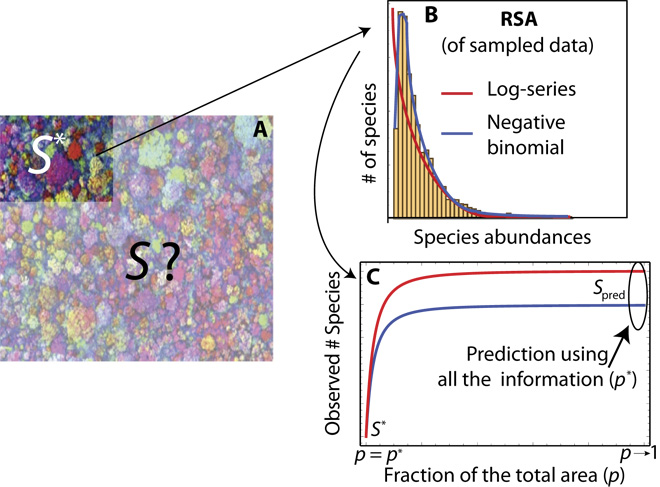
\includegraphics[width=0.6\linewidth]{Figure/RSA.jpg}
  \caption{\textbf{Rappresentazione schematica del modello di upscaling}. Questo consiste in tre passaggi. (\textbf{A}) Conosciamo l'abbondanza di $S^*$ specie alla scala di campionamento $\emph{p}^*$. (\textbf{B}) Facciamo un fit della SAD con una binomiale negativa o una distribuzione logaritmica. (\textbf{C}) Usando i parametri del miglior fit ottenuti in (B) e usando le equazioni (\ref{eq:SalphaLS}) e (\ref{eq:upscaleNB}) per dedurre la biodiversità dell'intero ecosistema.\cite{Tovoe1701438} }
  \label{fig:RSA1}
\end{figure}


\section{Metodo $Chao_\emph{wor}$}
Introduciamo ora il metodo non parametrico sviluppato da Chao, nato nell'ambito di uno schema di campionamento senza reinserimento. Il pedice \emph{wor} sta infatti per "\emph{without repetition}". Questo è il sistema di indagine più usato quando si devono campionare individui che non si desidera osservare ripetutamente (ad esempio nello studio delle foreste, nel quale gli alberi vengono censiti in piccole aree che sono selezionate senza ripetizione). In questo schema di campionamento ogni individuo o ogni unità di campionamento possono essere indagati una sola volta.\\
Assumiamo che in un ecosistema ci siano $S$ specie indicizzate da 1 a $S$.
Sia $N_\emph{i}$ (abbondanza assoluta) il numero di individui appartenenti alla \emph{i}-esima specie, \emph{i}=1,...,S, e $N_\emph{i}>0$. La popolazione totale dunque è data da $N=\sum_{\emph{i}=1}^{S} N_\emph{i}$. Assumiamo che la dimensione del campione $N$ sia nota, e che quindi sia nota anche la frazione di campionamento.\\
Supponiamo di prendere dall'intero ecosistema un campione di \emph{n} individui, campionandoli senza reinserimento. Sia $X_\emph{i}$ la frequenza della specie campionata cioè il numero di individui della \emph{i}-esima specie osservati nel campione. Solo le specie con  $X_\emph{i}>0$ sono osservabili nel campione. Sia $S^*_\emph{k}$ il numero di specie nel campione che sono rappresentate esattamente da \emph{k} individui, dunque $S^*_0$ denota il numero di specie che non sono state osservate nel campione. Dunque abbiamo che $\emph{n}=\sum_{\emph{i}=1}^S X_\emph{i}=\sum_{\emph{k}>1} \emph{k}S^*_\emph{k}$.
Definiamo $\emph{p}^*=\emph{n}/N$ la frazione di campionamento e $S^*$ il numero di specie osservate nel campione, $S^*=\sum_{\emph{k>1}} S^*_\emph{k}$.\\
Generalmente la probabilità che una specie venga rilevata, o rate di rilevamento, dipende sia dall'abbondanza della specie nel campione sia da caratteristiche specifiche degli individui come ad esempio il modo di spostarsi e muoversi all'interno dell'ambiente, colore, forma e dimensione.\\ Consideriamo dunque il caso generale in cui la probabilità di trovare un individuo possa variare a seconda della specie di appartenenza e indichiamola con $\theta_\emph{i}>0$ per la \emph{i}-esima specie.
Sotto queste ipotesi, definendo $\emph{p}_\emph{i}=N_\emph{i}/N $ come l'abbondanza relativa, il rate di rilevamento per la \emph{i}-esima specie diventa $\psi_{\emph{i}}=\frac{N_\emph{i}\theta_\emph{i}}{\sum_{\emph{k}=1}^S N_\emph{k}\theta_\emph{k}}=\frac{\emph{p}_\emph{i}\theta_\emph{i}}{\sum_{\emph{k}=1}^S \emph{p}_\emph{k}\theta_\emph{k}}$ con $\emph{i}=1,...,S$.
Intuitivamente, il numero di individui che hanno la stessa possibilità di essere osservati è dato da $N_\emph{i}\psi_\emph{i}$, ma poiché questo potrebbe essere un numero non intero, definiamo una variabile a valori interi $Z_\emph{i}$, che rappresenta il numero di individui che hanno la stessa possibilità di essere osservati per la \emph{i}-esima specie. Siccome $Z\ge 1$ e la frazione di individui campionata è $\emph{n}/N$, si può modellare il vettore \textbf{Z}=($Z_1,Z_2,...,Z_S$) attraverso una distribuzione multinomiale troncata di parametri N e  ($\psi_1^*,\psi_2^*,...,\psi_S^*$), dove $\psi_\emph{i}^* = \psi_i / P  \left\{\emph{z}:\emph{z}_\emph{i} \ge 1 , \emph{i}=1,...,S \right\} $, \textbf{z}=($\emph{z}_1 , \emph{z}_2,...,\emph{z}_S$) e $\sum_{\emph{i}=1}^S \emph{z}_\emph{i}=N$. Per ogni dato valore di \textbf{z}=($\emph{z}_1 , \emph{z}_2,...,\emph{z}_S$), le frequenze con cui appaiono gli individui della specie \emph{i}-esima nel campione, ($X_1,X_2,...,X_S$), seguono una distribuzione ipergeometrica generalizzata:
\\ \\
\begin{equation}
    P(X_\emph{i}=\emph{x}_\emph{i}, \emph{i}=1,2,...,S)=\binom{\emph{z}_1}{\emph{x}_1}\binom{\emph{z}_2}{\emph{x}_2}...\binom{\emph{z}_S}{\emph{x}_S}/\binom{N}{\emph{n}}
\end{equation}
$$ \emph{z}_\emph{i}\ge 1, \\ \sum_{\emph{i}=1}^S \emph{z}_\emph{i}=N.$$

Sulla base di questo modello generale, la distribuzione marginale per ognuna delle frequenze con le quali vengono individuate le specie è una distribuzione ipergeometrica:
\begin{equation}
P(X_\emph{i}=\emph{x}_\emph{i})=\binom{\emph{z}_\emph{i}}{\emph{k}}\binom{N-\emph{z}_\emph{i}}{\emph{n}-\emph{k}}/\binom{N}{\emph{n}}.
\label{eq:multinomial}
\end{equation}

\subsection{Il numero di specie a scala globale}
Vediamo dunque com'è possibile dedurre, sotto queste ipotesi, il numero di specie a scala globale a partire da un vettore di abbondanze ottenuto esaminando una frazione dell'intero ecosistema.\\ \\
Il valore di aspettazione per i contatori di frequenze $S^*_\emph{k}$ usando la (\ref{eq:multinomial}) è:
\begin{equation}
    \mathbb{E}(S^*_\emph{k})=\sum_\emph{i}^S P(X_\emph{i}=\emph{k})= \sum_{\emph{i}=1}^S \binom{\emph{z}_\emph{i}}{\emph{k}}\binom{N-\emph{z}_\emph{i}}{\emph{n}-\emph{k}}/\binom{N}{\emph{n}}
    \label{eq:expectationvalue}
\end{equation}

In particolare:
$$\mathbb{E}(S^*_0)=\sum_{\emph{i}=1}^S \binom{N-\emph{z}_\emph{i}}{\emph{n}}/\binom{N}{\emph{n}}$$

$$ \mathbb{E}(S^*_1)=\sum_{\emph{i}=1}^S \binom{\emph{z}_\emph{i}}{1} \binom{N-\emph{z}_\emph{i}}{\emph{n}-1}/\binom{N}{\emph{n}}=\sum_{\emph{i}=1}^S\frac{\emph{n}\emph{z}_\emph{i}}{N-\emph{z}_\emph{i}-\emph{n}+1} \binom{N-\emph{z}_\emph{i}}{\emph{n}}/\binom{N}{\emph{n}}$$



$$ \mathbb{E}(S^*_2)=\sum_{\emph{i}=1}^S \binom{\emph{z}_\emph{i}}{2} \binom{N-\emph{z}_\emph{i}}{\emph{n}-2}/\binom{N}{\emph{n}}=\sum_{\emph{i}=1}^S\frac{\emph{n}(\emph{n}-1)\emph{z}_\emph{i}(\emph{z}_\emph{i}-1)}{2(N-\emph{z}_\emph{i}-\emph{n}+1)(N-\emph{z}_\emph{i}-\emph{n}+2)} \binom{N-\emph{z}_\emph{i}}{\emph{n}}/\binom{N}{\emph{n}}$$

Per la disuguaglianza di Cauchy-Schwarz si ha:

$$
\left \{ \sum_{\emph{i}=1}^S\frac{\emph{n}\emph{z}_\emph{i}}{N-\emph{z}_\emph{i}-\emph{n}+1} \binom{N-\emph{z}_\emph{i}}{\emph{n}}/\binom{N}{\emph{n}} \right \}^2 \le $$ 
$$ \left \{ \sum_{\emph{i}=1}^S \binom{N-\emph{z}_\emph{i}}{\emph{n}}/\binom{N}{\emph{n}} \right \}\times \left \{ \sum_{\emph{i}=1}^S \left(\frac{\emph{n}\emph{z}_\emph{i}}{N-\emph{z}_\emph{i}-\emph{n}+1}\right)^2 \binom{N-\emph{z}_\emph{i}}{\emph{n}}/\binom{N}{\emph{n}} \right \},
$$
 dove vale il segno di uguaglianza quando tutte le $\emph{z}_\emph{i}$ sono uguali.
 
 La parte sinistra della disuguaglianza è $ \left \{ \mathbb{E}(S^*_1) \right \}^2$ e la prima sommatoria della parte destra è $ \left \{ \mathbb{E}(S^*_0) \right \}$. Per quanto riguarda la seconda sommatoria di destra riscrivendo:
 
 $$\left(\frac{\emph{n}\emph{z}_\emph{i}}{N-\emph{z}_\emph{i}-\emph{n}+1}\right)^2=\frac{\emph{n}}{\emph{n}-1}\left(\frac{\emph{n}(\emph{n}-1)\emph{z}_\emph{i}(\emph{z}_\emph{i}-1)}{(N-\emph{z}_\emph{i}-\emph{n}+1)^2}\right) + \frac{\emph{n}^2\emph{z}_\emph{i}}{(N-\emph{z}_\emph{i}-\emph{n}+1)^2} $$
 
essa diventa:

 
 $$\left \{ \sum_{\emph{i}=1}^S \left(\frac{\emph{n}\emph{z}_\emph{i}}{N-\emph{z}_\emph{i}-\emph{n}+1}\right)^2 \binom{N-\emph{z}_\emph{i}}{\emph{n}}/\binom{N}{\emph{n}} \right \} \approx \frac{2\emph{n}}{\emph{n}-1}\mathbb{E}(S^*_2)$$ 
 $$ + \sum_{\emph{i}=1}^S \left [ \frac{\emph{n}}{N-\emph{z}_\emph{i}-\emph{n}+1} \right ]\frac{\emph{n}\emph{z}_\emph{i}}{N-\emph{z}_\emph{i}-\emph{n}+1}\binom{N-\emph{z}_\emph{i}}{\emph{n}}/\binom{N}{\emph{n}}.$$
 \\
 Il contributo delle specie con $\emph{z}_\emph{i}$ grande  all'ultimo termine dell'equazione sopra è trascurabile, mentre per le specie con $\emph{z}_ \emph{i}$ molto più piccolo di $N$, abbiamo:
 
 $$
 \frac{\emph{n}}{N-\emph{z}_\emph{i}-\emph{n}+1}=\frac{\emph{n/N}}{(N-\emph{z}_\emph{i}-\emph{n}+1)/N} \approx \frac{\emph{n}/N}{1-\emph{n}/N}=\frac{\emph{p}^*}{1-\emph{p}^*}.
 $$
 
 Quindi otteniamo la seguente disuguaglianza:
 
$$
\left \{ \mathbb{E}(S^*_1) \right \}^2 \le \left \{ \mathbb{E}(S^*_0) \right \}\left \{ \frac{\emph{n}}{\emph{n}-1}2\mathbb{E}(S^*_2) + \frac{\emph{p}^*}{1-\emph{p}^*}\mathbb{E}(S^*_1) \right \},
$$

che è equivalente a:


\begin{equation}
\mathbb{E}(S^*_0) \ge \frac{\mathbb{E}({S^*_1}^2)}{\frac{\emph{n}}{\emph{n}-1}2\mathbb{E}(S^*_2)+ \frac{\emph{p}^*}{1-\emph{p}^*}\mathbb{E}(S^*_1)}.
\end{equation}

Sostituendo il valore di aspettazione con le frequenze osservate otteniamo come limite inferiore per la ricchezza delle specie:

\begin{equation}
    S_{\emph{p}=1}= S^* +\frac{{S^*_1}^2}{\frac{\emph{n}}{\emph{n}-1}2S^*_2+ \frac{\emph{p}^*}{1-\emph{p}^*}S^*_1}.
    \label{eq:chaoworestimator}
\end{equation}



% ---------------------  ESEMPI UTILI PRONTI ALL'USO  ----------------------------
%TERZO capitolo della tesi. Esempio di citazione doppia \cite{Munoz-Lipo,Vas}.
%
%Esempio di figura in \figurename\ \ref{FIG:LogoUniPD}.
%
%\begin{figure}[!htbp]
%\centering
%
\includegraphics[width=0.25\textwidth]{./figure//LogoUniPD}
%\caption{Esempio di figura.}
%\label{FIG:LogoUniPD}
%\end{figure}
%
%Esempio di tabella in \tablename\ \ref{TAB:Esempio}.
%
%\begin{table}[!htbp]
%\centering
%\renewcommand{\arraystretch}{1.3}
%\caption{Esempio di tabella.}
%\begin{tabular}{cc}
%\hline
%Nome & Valore \\
%\hline
%a & 1 \\
%b & 2 \\
%c & 3 \\
%d & 4 \\
%e & 5 \\
%f & 6 \\
%\hline
%\end{tabular}
%\label{TAB:Esempio}
%\end{table}

\clearemptydoublepage

\chapter{Applicazione della teoria ecologica alle comunità microbiche}

Gli ecosistemi di comunità microbiche presenti nel corpo umano giocano un ruolo molto importante per la nostra salute\cite{Costello1255}. Ogni individuo può essere visto come un insieme di habitat occupati da comunità microbiche formatesi attraverso i processi fondamentali dell'ecologia: diffusione, diversificazione locale, selezione ambientale e migrazione. I tanti e svariati membri delle comunità hanno un ruolo cruciale nel mantenimento della salute umana liberando essi nutrienti ed energia altrimenti inaccessibili, favorendo la differenziazione dei tessuti, stimolando il sistema immunitario e proteggendo l'ospite dall'invasione da parte di agenti patogeni. 
Un certo numero di disturbi clinici, come l'obesità, la malnutrizione e malattie infiammatorie, sono stati associati all'alterazione della composizione delle comunità microbiche presenti nell'ospite.\\
Il corpo umano, dunque, può essere visto come un ecosistema e la salute di un individuo può essere associata ai servizi forniti
all'organismo dalle comunità microbiche.\\
Recenti scoperte di variazioni inaspettate nella composizione del microbioma di individui sani hanno evidenziato l'importanza di identificare i processi che possano dare origine ad un tale cambiamento: la teoria dell'ecologia cerca di spiegare e predire questi fenomeni. Inoltre, il modello ecologico trasportato nel mondo delle pratiche cliniche può portare ad un miglioramento delle cure fornite ai pazienti: infatti, una visione completa della comunità che si va ad alterare con una certa terapia e non focalizzata solamente sul batterio a cui è dovuto il disturbo, può portare ad un nuovo approccio clinico che nella cura di una malattia tiene conto dell'intero microbioma dell'individuo.

\section{Sequenziamento del DNA degli individui in comunità microbiche}
Ottenere dati di biodiversità per una comunità microbica non è una cosa semplice: dopo averne prelevato una campione, per riconoscere le specie presenti al suo interno è necessario sequenziare il DNA in esso contenuto.\\
Lo sviluppo di tecniche di sequenziamento di nuova generazione (NGS, \emph{next-generation sequencing}) ha portato ad un incremento delle risorse impegnate in questo tipo di ricerca, aumentando rapidamente le nostre conoscenze sulla composizione e sulle funzioni delle popolazioni batteriche in diversi ambienti\cite{shotgun}. Nel contesto clinico, il microbioma dell'intestino umano è stato soggetto ad indagini sofisticate che hanno rivelato una forte interazione tra i microrganismi, il sistema immunitario e il metabolismo. Una ridotta biodiversità o uno squilibrio tra le popolazioni di specie batteriche all'interno comunità microbiche dell'intestino umano sono state associate ad una serie di fenotipi come l'obesità, malattie infiammatorie dell'intestino, diabete di tipo \RNum{2} e numerosi altri disturbi.\\
La maggior parte degli studi riguardanti la comprensione delle dinamiche che governano le popolazioni batteriche sono stati condotti attraverso i cosiddetti approcci metagenomici, che studiano cioè l'insieme dei diversi materiali genetici, in modo semplice ed efficace in termini di costi. I principali metodi di sequenziamento del DNA sono il metodo \emph{shotgun} e il metodo $16S$.
%Ci concentreremo ora sul metodo \emph{shotgun}, in quanto i dati che utilizzeremo successivamente in questo lavoro sono stati ottenuti attraverso questo metodo.
Il metodo \emph{shotgun} è una tecnica sperimentale di sequenziamento dell'intero genoma di un organismo\cite{HEATHER20161}. Poiché a causa dell'elevata lunghezza della sequenza genetica è impossibile sequenziare il genoma in un unico passaggio, esso consiste nella creazione di numerosi piccoli frammenti di DNA che vengono clonati e sequenziati separatamente da entrambi i versi. Questi poi vengono riassemblati \emph{in silico} attraverso criteri di compatibilità e sovrapposizione, in modo da ottenere una lunga sequenza continua. Con il metodo $16S$ invece si va a sequenziare il gene ribosomale $16S$ che da una parte, essendo contenuto in una regione molto conservata, aiuta l'amplificazione, e dall'altra parte,differendo da una specie all'altra, ne permette la classificazione.\\
Le sequenze così ottenute vengono poi confrontate con quelle presenti nei database che contengono le informazioni sui metagenomi dei batteri finora sequenziati. In particolare il progetto microbioma umano (HMP, \emph{human microbiome project}) contiene una vasta raccolta di sequenze di microorganismi associati al corpo umano, inclusi eucarioti, batteri, archei e virus, ottenute sia con il metodo \emph{shotgun} che con il sequenziamento $16S$. Attingendo a queste informazioni è dunque possibile ottenere informazioni su quali specie batteriche siano presenti all'interno di campioni di interesse e con quali abbondanze.



\section{Applicazione dei metodi di \emph{upscaling}}
Dato un campione di $N$ individui (cioè, nel caso di dati metagenomici, di $N$ sequenze di DNA, ovvero i cosiddetti \emph{reads}), grazie ai metodi di classificazione tassonomica sopra citati, è possibile assegnare la specie solamente ad una frazione di questi; le restanti sequenze vengono scartate perché non risultano esserci  batteri con tali stringhe di DNA nel database di riferimento. Analogamente a quanto viene fatto in ecologia, utilizzando i metodi \emph{upscaling} si potrebbe usare tale frazione $p^*$ per capire quante specie erano in realtà presenti nell'intero campione. Questa $p^*$ può essere stimata come il rapporto tra il numero di sequenze che hanno trovato riscontro nel database, $N^*$, e il numero di sequenze inizialmente presenti nel campione, $N$, dunque $p^*=N^*/N$.  Le specie assenti nel campione di riferimento in ecologia corrispondono quindi, in questo contesto, alle specie a cui appartengono le sequenze che non riescono ad essere classificate.

Per questo lavoro sono stati ottenuti, utilizzando il software Kaiju\cite{Kaiju}, due vettori di abbondanze batteriche a partire da campioni sequenziati con metodo \emph{shotgun}. In particolare un campione riguarda il microbioma un individuo sano mentre l'altro riguarda quello di un individuo affetto dal morbo di Crohn, una malattia dell'intestino. I dati utilizzati sono stati presi dallo studio svolto nell'articolo "Characterization of the gut microbiome using 16S or shotgun metagenomics"\cite{shotgun}. \\

\subsection{Test}
Per sondare l'efficienza nell'ambito delle comunità microbiche dei metodi di \emph{upscaling} precedentemente descritti sono stati condotti dei test su ognuno dei due campioni, procedendo in questo modo:
\begin{itemize}
    \item per ogni campione sono stati selezionati 100 sottocampioni in modo casuale, ognuno contenete l'$1\%$ della popolazione totale;
    
    \item ad ogni sottocampione sono stati applicati i metodi di \emph{upscaling}, i due parametrici della binomiale negativa e della distribuzione logaritmica e il metodo non parametrico $\emph{Chao}_\emph{wor}$, con con $p^*=0.01$;
    
    \item sono stati predetti i numeri di specie alla scala globale (quella del campione) e confrontati con quelli reali che conosciamo a tale scala.
\end{itemize}

Analizzando i risultati dei test abbiamo notato i seguenti fatti:
\begin{itemize}
    \item il metodo $\emph{Chao}_\emph{wor}$ è inapplicabile. Questo infatti si basa sul conteggio del numero di specie rare, popolate cioè da uno o due individui. Nel caso di comunità microbiche non vengono identificate specie con questo tipo di caratteristiche alla sotto-scala analizzata e dunque il metodo non fornisce alcun risultato;
    
    \item il metodo parametrico della distribuzione logaritmica di Fisher sovrastima il numero di specie, in particolare predice circa il doppio del numero di specie realmente presenti nel campione iniziale;
    
    \item il metodo parametrico della binomiale negativa fornisce in tutti i casi analizzati una stima corretta del numero di specie presenti nel campione.
    
\end{itemize}

Alla luce dei risultati dei test applichiamo ai nostri campioni solo i due metodi parametrici.\newline

%\begin{table}[]
%\centering
%\begin{tabular}{l|l|l|l|l|}
%\cline{2-5}
%                                     & \textbf{nSpecie} & \textbf{LS} & \textbf{NB} & \textbf{Chao}
%                         \\ \hline
%\multicolumn{1}{|l|}{\textbf{Sano}}  & 43               & 78          & 43          & non applicabile        \\ \hline
%\multicolumn{1}{|l|}{\textbf{Crohn}} & 34.7              & 68          & 34          & non applicabile        \\ \hline
%\end{tabular}
%\caption{Simulazione Sniper Attack}
%\label{Tab:sniperattack}
%\end{table}

\subsection{Risultati di \emph{upscaling}}
Nelle seguenti figure sono rappresentate le RSA dei due campioni. (DESCRIVERE IL TIPO DI GRAFICI Preston Plot)


\begin{figure}[H]
  \centering
  \begin{minipage}[b]{0.4\textwidth}
    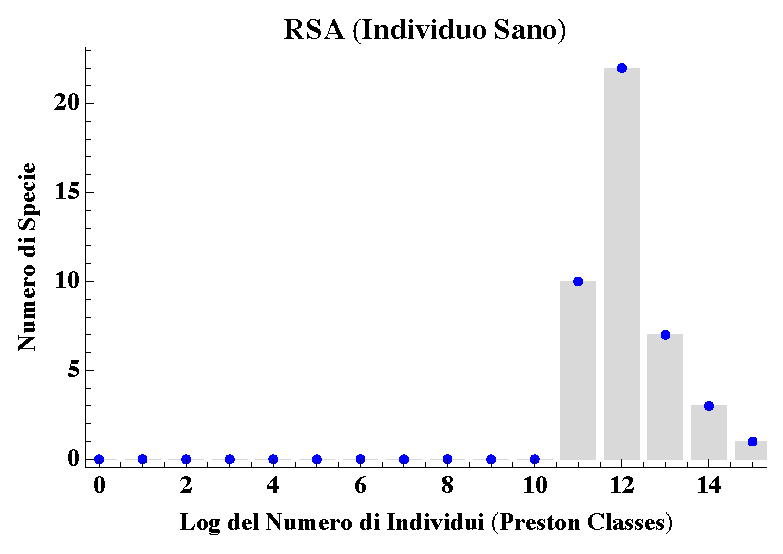
\includegraphics[width=\textwidth]{Figure/RSAH.eps}
    \caption{RSA individuo sano.}
    \label{fig:RSAH}
  \end{minipage}
  \hfill
  \begin{minipage}[b]{0.4\textwidth}
    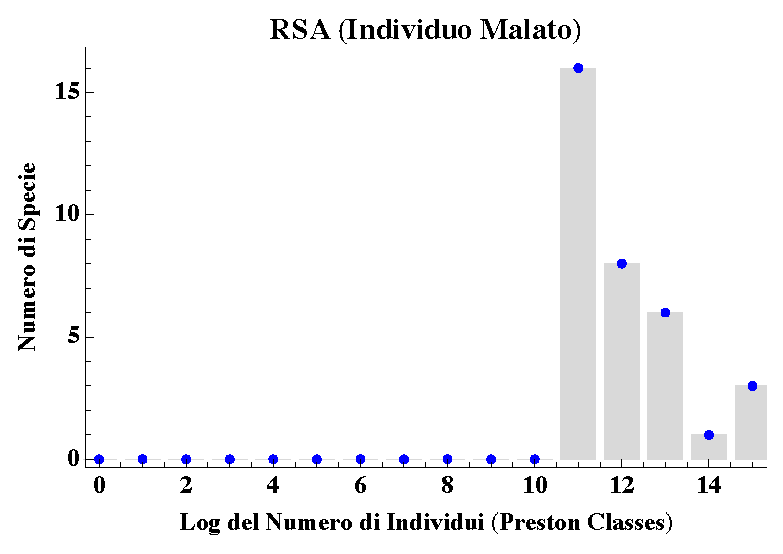
\includegraphics[width=\textwidth]{Figure/RSAC.eps}
    \caption{RSA individuo malato.}
    \label{fig:RSAC}
  \end{minipage}
\end{figure}

\begin{table}[H]
\centering
\begin{tabular}{l|l|l|l|l|}
\cline{2-5}
                                     & $\mathbf{S^*}$ & $\mathbf{N^*}$ & $\mathbf{N}$ & $\mathbf{p^*}$ \\ \hline
\multicolumn{1}{|l|}{\textbf{Sano}}  & 43                & 176531               & 733551           & 0.240653    \\ \hline
\multicolumn{1}{|l|}{\textbf{Crohn}} & 34                & 159376               & 268205           & 0.594232    \\ \hline
\end{tabular}
\caption{Dati Iniziali.}
\label{Tab:dati}
\end{table}

Nella tabella \ref{Tab:dati} sono indicati, per ognuno dei due campioni, il numero di specie $S^*$ e di individui $N^*$ riconosciuti, il numero di sequenze $N$ ricostruite prima che venissero scartate quelle che non hanno trovato riscontro nel database e la $p^*$ corrispondente, stimata come $p^*=N^*/N$.


Assumendo per la RSA una forma binomiale negativa e fittando il corrispondente pattern empirico otteniamo i seguenti parametri:


\begin{table}[H]
\centering
\begin{tabular}{l|l|l|l|}
\cline{2-4}
                                     & \textit{r}    & $\mathbf{\hat \xi}_{p^*}$                & $\mathbf{\xi}$             \\ \hline
\multicolumn{1}{|l|}{\textbf{Sano}}  & $2.4 \pm 0.4$ & $0.9994 \pm 0.0001$ & $0.999861 \pm $ \\ \hline
\multicolumn{1}{|l|}{\textbf{Crohn}} & $1.2 \pm 0.3$ & $0.999752 \pm $     & $0.9999 \pm 0.00007$ \\ \hline
\end{tabular}
\caption{Parametri Binomiale Negativa.}
\label{Tab:dati}
\end{table}

assumendo invece una distribuzione logaritmica otteniamo:


(TABELLA??)

Il numero di specie predetto da ognuno dei due modelli è riportato nella seguente tabella:

(TABELLA)

(GRAFICI CON CURVE)

\clearemptydoublepage


\phantomsection
%\addcontentsline{toc}{chapter}{Considerazioni finali}
\chapter{Conclusioni}


%------------------------------------------------------------------------------------
%Le conclusioni devono essere brevi e comporsi dei seguenti punti:
%\begin{itemize}
%\item indicazione di ci� che si � esposto e del suo significato
%\item analisi comparativa e commento critico dei risultati presentati
%\item spiegazione motivata delle parti omesse o non approfondite
%\item indicazione dei possibili ulteriori sviluppi.
%\end{itemize}
%------------------------------------------------------------------------------------


% ---------------------  ESEMPI UTILI PRONTI ALL'USO  ----------------------------
%TERZO capitolo della tesi. Esempio di citazione doppia \cite{Munoz-Lipo,Vas}.
%
%Esempio di figura in \figurename\ \ref{FIG:LogoUniPD}.
%
%\begin{figure}[!htbp]
%\centering
%
\includegraphics[width=0.25\textwidth]{./figure//LogoUniPD}
%\caption{Esempio di figura.}
%\label{FIG:LogoUniPD}
%\end{figure}
%
%Esempio di tabella in \tablename\ \ref{TAB:Esempio}.
%
%\begin{table}[!htbp]
%\centering
%\renewcommand{\arraystretch}{1.3}
%\caption{Esempio di tabella.}
%\begin{tabular}{cc}
%\hline
%Nome & Valore \\
%\hline
%a & 1 \\
%b & 2 \\
%c & 3 \\
%d & 4 \\
%e & 5 \\
%f & 6 \\
%\hline
%\end{tabular}
%\label{TAB:Esempio}
%\end{table}

%\backmatter

\clearemptydoublepage

%\phantomsection
\addcontentsline{toc}{chapter}{Ringraziamenti}
\chapter*{Ringraziamenti}

Eventuali ringraziamenti personali. % non obbligatorio
%\clearemptydoublepage

\bibliographystyle{IEEEtran}
%\bibliography{IEEEabrv,./7-Bibliografia/Biblio}

\begin{thebibliography}{9} 

\bibitem{tor} R. Dingledine, N. Mathewson, and P. Syverson,\textit{"TOR: The second-generation onion router,"} In USENIX Security Symposium (San Diego, CA, 2004), USENIX Association, pp. 303-320.

\bibitem{tormetrics} Tor Metrics \url{https://metrics.torproject.org/}, [Accesso: 13 Settembre 2016].

\bibitem{torspec} Tor's protocol specifications \url{https://gitweb.torproject.org/torspec.git/tree/dir-spec.txt}, [Accesso: 13 Settembre 2016].

\bibitem{torbridge} Z. Ling, J. Luo, W. Yu, M. Yang, and X. Fu,\textit{"Extensive analysis and large-scale empirical evaluation of Tor bridge discovery,"} in Proc. IEEE INFOCOM, 2012, pp. 2381-2389.

\bibitem{gfc} P. Winter, S. Lindskog, \textit{"How the Great Firewall of China is Blocking Tor,"} Free and Open Communications on the Internet, 2012.

\bibitem{meek} The Tor Project. Meek \url{https://trac.torproject.org/projects/tor/wiki/doc/meek}, [Accesso: 13 Settembre 2016].

\bibitem{domainfronting} D. Fifield, C. Lan, R. Hynes, P. Wegmann, and V. Paxson, \textit{"Blocking-resistant communication through domain fronting,"} Proceedings on Privacy Enhancing Technologies 2015, pp. 1-19.

\bibitem{cellflood} M. V. Barbera, V. P. Kemerlis, V. Pappas, and A. Keromytis, \textit{"CellFlood: Attacking Tor Onion Routers on the Cheap,"} in Proc. ESORICS, Sep. 2013, pp. 664-681.

\bibitem{sniper} R. Jansen, F. Tschorsch, A. Johnson, and B. Scheuermann, \textit{"The sniper attack: Anonymously deanonymizing and disabling the Tor network,"} in Proc. 21st Annu, Symp. NDSS, Feb. 2014, pp. 1-15.

\bibitem{packetspinning} V. Pappas, E. Athanasopoulos, S. Ioannidis, and E. P. Markatos,\textit{"Compromising Anonymity Using Packet Spinning,"} in ISC 08, Sep. 2008.

\bibitem{lochidd} Lasse {\O}verlier and Paul Syverson, \textit{"Locating Hidden Servers,"} in Proceedings of the IEEE Security and Privacy Symposium (S\&P), May 2006.

\bibitem{survey} E. Erdin, C. Zachor, and M. H. Gunes, \textit{"How to Find Hidden Users: A Survey of Attacks on Anonymity Networks,"}. IEEE Commun. Surv. Tutorials, vol. 17, no. 4, pp. 2296-2316, 2015.

\end{thebibliography}

\appendix

\clearemptydoublepage

%\chapter{(se necessaria)}

Allo scopo di rendere pi� scorrevole la lettura del corpo dell'elaborato, in appendice pu�
essere opportuno riportare:
\begin{itemize}
\item i passaggi matematici non essenziali
\item le dimostrazioni di teoremi
\item le tabelle con i risultati di campagne di misure i cui grafici sono inseriti nel corpo
dell'elaborato
\item i listati dei programmi di calcolo
\item i ``data sheet'' di componenti cui si fa riferimento nel testo principale.
\end{itemize} % non obbligatorio
%\clearemptydoublepage

% Lista delle figure (non obbligatoria)
\listoffigures

\clearemptydoublepage

% Lista delle tabelle (non obbligatoria)
\listoftables

\clearemptydoublepage


% Ridefiniamo l'etichetta per le figure e le tabelle
\renewcommand{\figurename}{Fig.}
\renewcommand{\tablename}{Tab.}
% Ridefiniamo percentuali per inserimento figure nel testo
\renewcommand{\topfraction}{0.85}
\renewcommand{\textfraction}{0.1}
\renewcommand{\floatpagefraction}{0.75}

\bibliography{7-Bibliografia/Biblio}{}
\bibliographystyle{plain}
\end{document}